
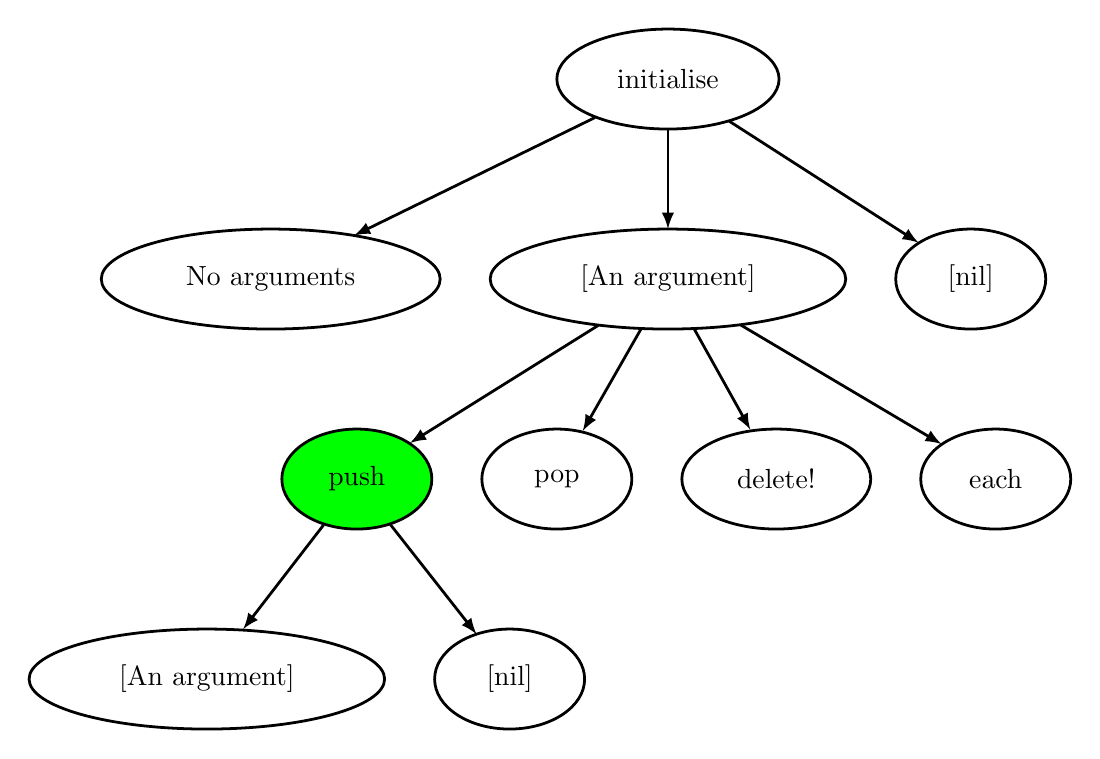
\begin{tikzpicture}[>=latex,line join=bevel,]
  \pgfsetlinewidth{1bp}
%%
\pgfsetcolor{black}
  % Edge: b1 -> c2
  \draw [->] (128.93bp,73.811bp) .. controls (136.21bp,64.546bp) and (145.66bp,52.52bp)  .. (160.09bp,34.159bp);
  % Edge: initialise -> a3
  \draw [->] (251.06bp,218.83bp) .. controls (268.27bp,207.78bp) and (292.27bp,192.36bp)  .. (319.24bp,175.05bp);
  % Edge: b1 -> c1
  \draw [->] (105.02bp,73.465bp) .. controls (98.316bp,64.78bp) and (89.807bp,53.75bp)  .. (76.085bp,35.962bp);
  % Edge: initialise -> a2
  \draw [->] (229bp,215.7bp) .. controls (229bp,207.98bp) and (229bp,198.71bp)  .. (229bp,180.1bp);
  % Edge: initialise -> a1
  \draw [->] (202.77bp,220.16bp) .. controls (181.04bp,209.52bp) and (149.82bp,194.24bp)  .. (116.02bp,177.7bp);
  % Edge: a2 -> b4
  \draw [->] (255.19bp,145.46bp) .. controls (274.06bp,134.27bp) and (299.5bp,119.18bp)  .. (327.49bp,102.58bp);
  % Edge: a2 -> b2
  \draw [->] (219.32bp,144.05bp) .. controls (214.53bp,135.68bp) and (208.66bp,125.4bp)  .. (198.32bp,107.31bp);
  % Edge: a2 -> b3
  \draw [->] (238.44bp,144.05bp) .. controls (243.04bp,135.8bp) and (248.67bp,125.7bp)  .. (258.65bp,107.79bp);
  % Edge: a2 -> b1
  \draw [->] (203.87bp,145.29bp) .. controls (186.4bp,134.38bp) and (163.11bp,119.82bp)  .. (136.13bp,102.96bp);
  % Node: b4
\begin{scope}
  \definecolor{strokecol}{rgb}{0.0,0.0,0.0};
  \pgfsetstrokecolor{strokecol}
  \draw (347bp,90bp) ellipse (27bp and 18bp);
  \draw (347bp,90bp) node {each};
\end{scope}
  % Node: a1
\begin{scope}
  \definecolor{strokecol}{rgb}{0.0,0.0,0.0};
  \pgfsetstrokecolor{strokecol}
  \draw (86bp,162bp) ellipse (61bp and 18bp);
  \draw (86bp,162bp) node {No arguments};
\end{scope}
  % Node: a3
\begin{scope}
  \definecolor{strokecol}{rgb}{0.0,0.0,0.0};
  \pgfsetstrokecolor{strokecol}
  \draw (338bp,162bp) ellipse (27bp and 18bp);
  \draw (338bp,162bp) node {[nil]};
\end{scope}
  % Node: initialise
\begin{scope}
  \definecolor{strokecol}{rgb}{0.0,0.0,0.0};
  \pgfsetstrokecolor{strokecol}
  \draw (229bp,234bp) ellipse (40bp and 18bp);
  \draw (229bp,234bp) node {initialise};
\end{scope}
  % Node: b1
\begin{scope}
  \definecolor{strokecol}{rgb}{0.0,0.0,0.0};
  \pgfsetstrokecolor{strokecol}
  \definecolor{fillcol}{rgb}{0.0,1.0,0.0};
  \pgfsetfillcolor{fillcol}
  \filldraw [opacity=1.0] (117bp,90bp) ellipse (27bp and 18bp);
  \draw (117bp,90bp) node {push};
\end{scope}
  % Node: b2
\begin{scope}
  \definecolor{strokecol}{rgb}{0.0,0.0,0.0};
  \pgfsetstrokecolor{strokecol}
  \draw (189bp,90bp) ellipse (27bp and 18bp);
  \draw (189bp,90bp) node {pop};
\end{scope}
  % Node: b3
\begin{scope}
  \definecolor{strokecol}{rgb}{0.0,0.0,0.0};
  \pgfsetstrokecolor{strokecol}
  \draw (268bp,90bp) ellipse (34bp and 18bp);
  \draw (268bp,90bp) node {delete!};
\end{scope}
  % Node: c2
\begin{scope}
  \definecolor{strokecol}{rgb}{0.0,0.0,0.0};
  \pgfsetstrokecolor{strokecol}
  \draw (172bp,18bp) ellipse (27bp and 18bp);
  \draw (172bp,18bp) node {[nil]};
\end{scope}
  % Node: c1
\begin{scope}
  \definecolor{strokecol}{rgb}{0.0,0.0,0.0};
  \pgfsetstrokecolor{strokecol}
  \draw (63bp,18bp) ellipse (64bp and 18bp);
  \draw (63bp,18bp) node {[An argument]};
\end{scope}
  % Node: a2
\begin{scope}
  \definecolor{strokecol}{rgb}{0.0,0.0,0.0};
  \pgfsetstrokecolor{strokecol}
  \draw (229bp,162bp) ellipse (64bp and 18bp);
  \draw (229bp,162bp) node {[An argument]};
\end{scope}
%
\end{tikzpicture}

